% aspectratio: 43 for old style 4:3, 169 for wide screen 16:9
% If you don't know if the screen will be wide screen or 4:3 you can use
% 1610 for a compromise to have smaller borders on either of the usual aspect ratios
% \documentclass[aspectratio=169,9pt]{beamer}
\documentclass[
aspectratio=169,
14pt,
professionalfonts
]{beamer}

\usetheme[patchframe=true]{LMU}

% \usepackage{fontspec}
% \setsansfont{Source Sans Pro}
% \setmonofont{Fira Code}[Contextuals=Alternate]

% \usepackage{mathspec}

\renewcommand*{\thefootnote}{\fnsymbol{footnote}}

\newcommand\identity{1\kern-0.25em\text{l}}

\newcommand{\pyhf}{\texttt{pyhf}\xspace}

\newcommand{\arrow}{~\ding{220}~}

\DeclareMathOperator\supp{supp}

\title[]{Bayesian inference in particle physics}

\author[L. G\"artner]{\underline{Lorenz G\"artner}$^{1}$, Toni Sculac, Judith Katzy }

\institute[LMU]{$^1$LMU Munich}

\date{\today}

\begin{document}

\begin{frame}[titleslide]
    \titlepage
    \begin{tikzpicture}[remember picture,overlay]
    \node[anchor=south west, yshift=2mm, xshift=2mm] at (current page.south west)
    {%
      
\includegraphics[height=1.cm]{common/logos/origins.pdf}
      
\includegraphics[height=1.cm]{common/logos/belle2.pdf}
      
\includegraphics[height=1.cm]{common/logos/punch4nfdi.png}
      
\includegraphics[height=1.cm]{common/logos/dfg.jpg}
      % 
\includegraphics[height=1.5cm]{common/logos/bmbf.pdf}
    };%
    \end{tikzpicture}
\end{frame}

\begin{frame}

\centering
\Large
What is a probability?
    
\end{frame}

\begin{frame}{Kolmogorov's probability axioms}
% https://plato.stanford.edu/entries/probability-interpret/#MaiInt
\begin{enumerate}
  \item $ p(\Omega) = 1 $, where \( \Omega \) is the sample space.
  \item $ p(x) \geq 0 $ for any event \( x \subseteq \Omega \).
  \item For any sequence of disjoint events \( x_1, x_2, \dots \), 
        $$
        p\left( \bigcup_{i=1}^{\infty} x_i \right) = \sum_{i=1}^{\infty} p(x_i)
        $$
\end{enumerate}
\end{frame}


\begin{frame}{Conditional probability}
Is \textbf{defined} as the probability of an event $x$ if we know that an event $y$ is true
$$p(x|y) = \frac{p(x \cup y)}{p(y)}$$
\end{frame}

\begin{frame}{Probability interpretations}
    The probability axioms and probability rules allow you to calculate new probabilities from old ones. 

    But axioms do not tell you how to assign probabilities to begin with. For this we need probability interpretations. 

    The interpretations share the same mathematical framework, but the meaning of $p(x)$ is different.
\end{frame}

\begin{frame}{Frequentist interpretation}
Assign a probability as relative frequency
$$
p(x) = \lim_{n\to\infty} \frac{n_x}{n}
$$ 

\begin{itemize}
    \item Can only be assigned to repeatable experiments
    \item Not everything is repeatable...
    \item No probabilities of single events
\end{itemize}
\end{frame}

\begin{frame}{Bayesian interpretation}
Assign a probability $p(x)$ as \textit{degree of belief}.

\begin{itemize}
    \item Probability depends on the experimenters' knowledge.
    \item Inference results are subjective.
    \item Everything is a random variable.
\end{itemize}
\end{frame}

\begin{frame}{Bayesian inference}

The Bayesian posterior is

$$p(\text{theory} | \text{data}) = \frac{p(\text{data}|\text{theory}) p(\text{theory})}{p(\text{data})}$$

\begin{itemize}
    \item \textbf{Likelihood} $p(\text{data}|\text{theory})$
    \item \textbf{Prior} $p(\text{theory})$
    \item \textbf{Evidence} $p(\text{data}) = \int p(\text{data}|\text{theory}) p(\text{theory}$
\end{itemize}
\end{frame}

\begin{frame}{The common ground}
\textbf{Frequentist inference} is based on 
\begin{itemize}
    \item the model of the observable data \textbf{$$p(x|\theta)$$}
\end{itemize}
\textbf{Bayesian inference} is based on 
\begin{itemize}
    \item the model of the observable data \textbf{$$p(x|\theta)$$}
    \item your prior belief $$p(\theta)$$
\end{itemize}
\end{frame}

\begin{frame}{Physics does not care...}{... about our interpretation}
For many inference problems, the frequentist and Bayesian approaches give similar numerical
values, even though they answer different questions and are based on fundamentally different interpretations of probability.

Pour all energy into constructing the best possible \textbf{$p(x|\theta)$}
\end{frame}

\begin{frame}{Bayesian updating}
Parameter values $\theta$ under which data $x_1, x_2$ is more probable on average get weighted up, other values get weighted down.
$$
p(\theta | x_1, x_2) = \frac{p(x_2|\theta)}{p(x_2)} \frac{p(x_1|\theta)}{p(x_1)} p(\theta)
$$
\end{frame}

\begin{frame}{Bayesian updating}
% \vspace{-1cm}
\begin{figure}
    \centering
    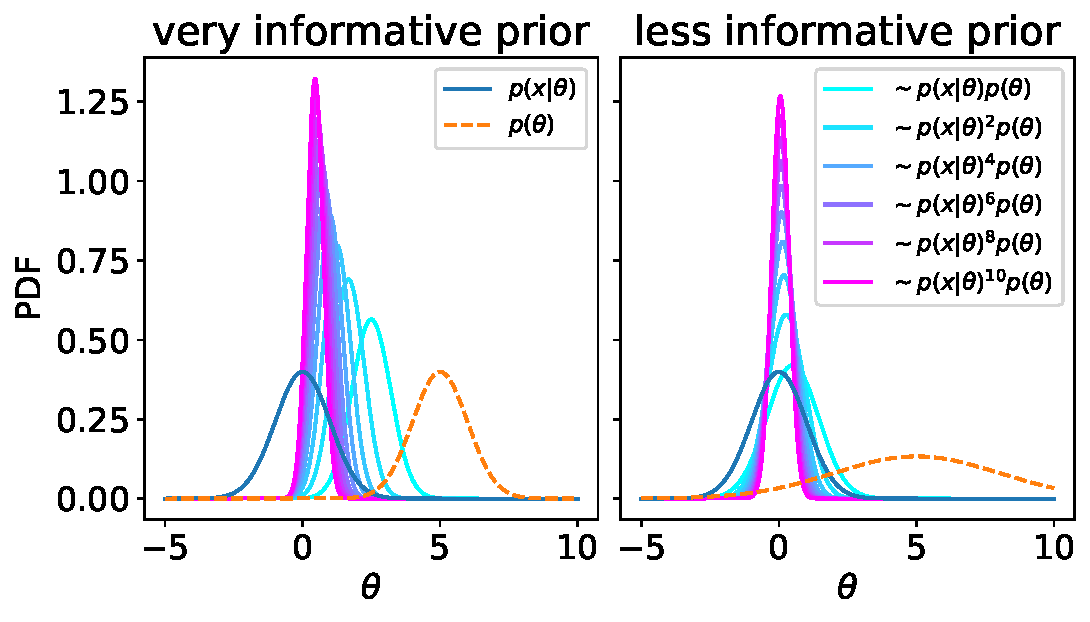
\includegraphics[width=0.9\linewidth]{../plots/updating.pdf}
\end{figure}
\end{frame}

\begin{frame}
\center
\Large
Nuisance parameters and priors
\end{frame}

\begin{frame}{Frequentist nuisance parameters}

Models are not perfect \arrow \textbf{systematic bias} 

More general models include additional \textbf{nuisance} parameters, $\nu$,
$$p(x|\theta, \nu)$$

Leads to increased statistical uncertainties on POIs (due to correlation)

Want to constrain nuisance parameters, but in the frequentist language \textbf{everything is data}.


% In general the model is not perfect, which is to say it cannot provide an accurate description of the data even at the most optimal point of its parameter space. As a result, the estimated parameters can have a systematic bias.

% Although including additional parameters may eliminate or at least reduce the effect of systematic uncertainties, their presence will result in increased statistical uncertainties for the parameters of interest. This occurs because the estimators for the nuisance parameters and those of interest will in general be correlated, which results in an enlargement of the contour defined by Eq. (40.13).

% To reduce the impact of the nuisance parameters one often tries to constrain their values by means of control or calibration measurements, say, having data y. 

% L(θ, ν) = P (x|θ, ν)P (y|ν) . 

% Note that in this case if one wants to simulate the experiment by means of Monte Carlo, both the primary and control measurements, x and y, must be generated for each repetition under assumption of fixed values for the parameters θ and ν.

% Using all of the parameters (θ, ν) in Eq. (40.13) to find the statistical errors in the parameters of interest θ is equivalent to using the profile likelihood, which depends only on θ. It is defined as Lp(θ) = L(θ,̂̂ ν(θ)), 

\end{frame}

\begin{frame}{... everything is data}    
    "\textit{The great advantage of the Bayesian approach is that it allows you to incorporate subjective beliefs, while the Frequentist approach pretends that you don't have any.}" 
    \flushright -- associated with Jim Berger by ChatGPT
\end{frame}

\begin{frame}{... everything is data}    

    

    % We have a lot of prior knowledge, to just ignore it would be mad.

    {\centering Are we being honest here?}
    
    Prior knowledge in a typical frequientist analysis
    \begin{itemize}
        \item theory predictions
        \item model parameters (masses, couplings, ...)
        \item missing higher-order corrections
        \item MC normalizations
        \item ...
    \end{itemize}
    % https://indico.cern.ch/event/243641/attachments/415317/577061/CERN-Stat-Lectures.pdf
\end{frame}

\begin{frame}{Frequentist "priors"}
Constrain nuisance parameters using "auxiliary data" $a$,
$$L(\theta, \nu) = p(x| \theta, \nu) p(a| \nu)$$

$p(a, \nu)$ represents our "degree of belief" in $\nu$.

\vspace{0.5cm}

Often "auxiliary data" is \textit{created} to match our desired constraint term.
\end{frame}

\begin{frame}{Bayesian nuisance parameters}
If one has auxiliary data, the prior is
$$p(\nu|a) \propto p(a|\nu) p_0(\nu)$$
If $p_0(\nu)$ is chosen to have minimal impact, this overlaps with the frequentist treatment.

In the Bayesian case, other prior choices are also allowed, e.g.
$$ p(\nu) = \text{Gauss}(\nu | \nu_0, \sigma_\nu)$$

Bayesian approach also requires priors for POIs.
\end{frame}

\begin{frame}
\center
\Large
Parameter inference
\end{frame}

\begin{frame}{Parameter inference}
    \center
    \textbf{Point estimates}\\
    Identify the most probable parameter point.
    
    \vspace{1cm}
    
    \textbf{Interval estimation}\\
    Identify extended regions in parameter space based on compatibility with the data.
\end{frame}

\begin{frame}{Frequentist point estimates: estimators}
    Estimator is a \textit{statistic} $\hat \theta(x)$, i.e. a well chosen function of the data. \\
    Desired properties
    \begin{itemize}
        \item \textit{consistency} $\lim_{N_x \to \infty} E(\hat \theta) = \theta_{true}$
        % converges toward true value as number of observations increase
        \item \textit{unbiasedness} $b = E(\hat \theta) - \theta_{true}$
        % 
        \item \textit{efficiency} (minimum variance)
        \item ...
    \end{itemize}
    %TODO include graphic from James p 130
\end{frame}

\begin{frame}{A good data set is the key to success ...}
\begin{figure}
    \centering
    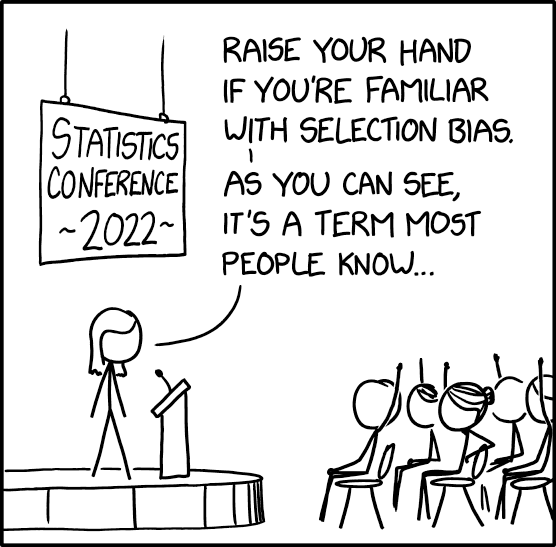
\includegraphics[width=0.4\linewidth]{../plots/selection_bias_2x.png}
\end{figure}
\end{frame}

\begin{frame}{Method of maximum likelihood}
    We find maximum likelihood estimators $ \hat \theta$ by solving
    $$
    \frac{\partial \ln L(x|\theta)}{\partial \theta}\mid_{\theta = \hat \theta} = 0
    $$
    With the property
    $$
    \lim_{N \to \infty} p\left(\sqrt{N}(\hat \theta - \theta_{true})\right) = \mathcal{N}(0, I^{-1}(\theta))
    $$
    This implies consistency, asymptotic unbiasedness and efficiency
    $$ \lim_{N \to \infty} V(\hat \theta) = I(\theta)^{-1} = E\left[\frac{\partial \ln L(x|\theta)}{\partial \theta}\right]^{-1}$$
\end{frame}

% \begin{frame}{Asymptotic normality}
%     In the asymptotic limit $N \to \infty$ they have the properties of
%     $$
%     lim_{N_x \to \infty} \sqrt{N}(\hat \theta - \theta_{true}) \sim \mathcal{N}(0, I^{-1}(\theta))
%     $$
%     \begin{itemize}
%         \item \textit{consistency}
%         \item \textit{efficiency}: variance given by Cramer-Rao bound
%         $$ \lim_{N_x \to \infty} V(\hat \theta) = E\left[\frac{\partial \ln L(x|\theta)}{\partial \theta}\right]^{-1}$$
%         \item \textit{robustness}: asymptotically Normal
%     \end{itemize}
% \end{frame}

\begin{frame}{Bayesian point estimates}
    \begin{minipage}{0.49\textwidth}
        \textbf{Mode / MAP}\\ Value of $\theta$ with maximum a-posteriori probability
            $$\theta_{MAP} = \text{argmax}_\theta ~ p(\theta|x)$$
        \textbf{Mean}\\ Expected value of $\theta$ under the posterior
            $$ \bar{\theta} = E_{p(\theta|x)}[\theta]$$
    \end{minipage}
    \begin{minipage}{0.49\textwidth}
        \begin{figure}
            \centering
            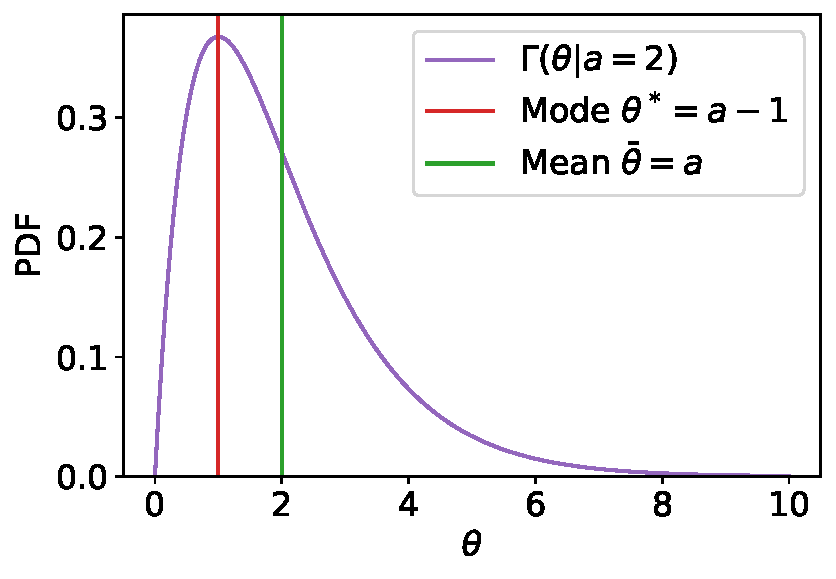
\includegraphics[width=\linewidth]{../plots/map_vs_mean.pdf}
        \end{figure}
    \end{minipage}
\end{frame}

\begin{frame}{Intervals and limits}
\begin{figure}
    \centering
    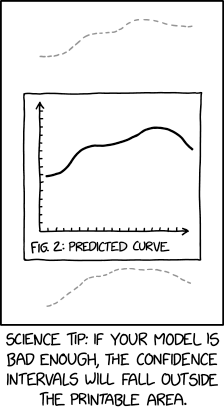
\includegraphics[width=0.25\linewidth]{../plots/confidence_interval.png}
    %https://xkcd.com/2311
\end{figure}
\end{frame}

\begin{frame}{Intervals and limits}
If an estimator PDF is not Normal, $\hat \theta \pm \sigma_\theta$ is meaningless.

\begin{figure}
    \centering
    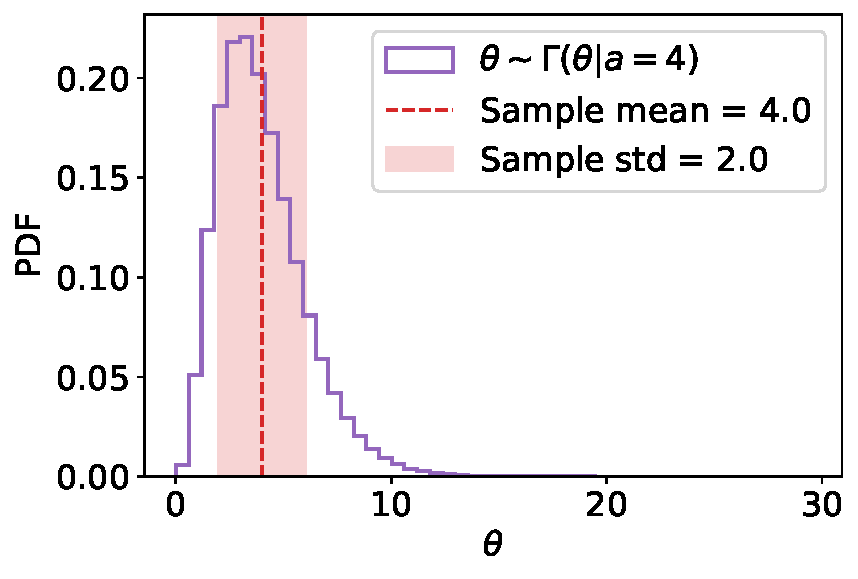
\includegraphics[width=0.6\linewidth]{../plots/gamma.pdf}
\end{figure}
    
\end{frame}

\begin{frame}{Frequentist intervals}

\begin{minipage}[t]{0.49\linewidth}
\textbf{Neyman confidence belt}
$$
\int_{x_1}^{x_2} dx ~ p(x|\theta) \geq 1-\alpha
$$
\end{minipage}
\begin{minipage}[t]{0.49\linewidth}
\begin{figure}
    \centering
    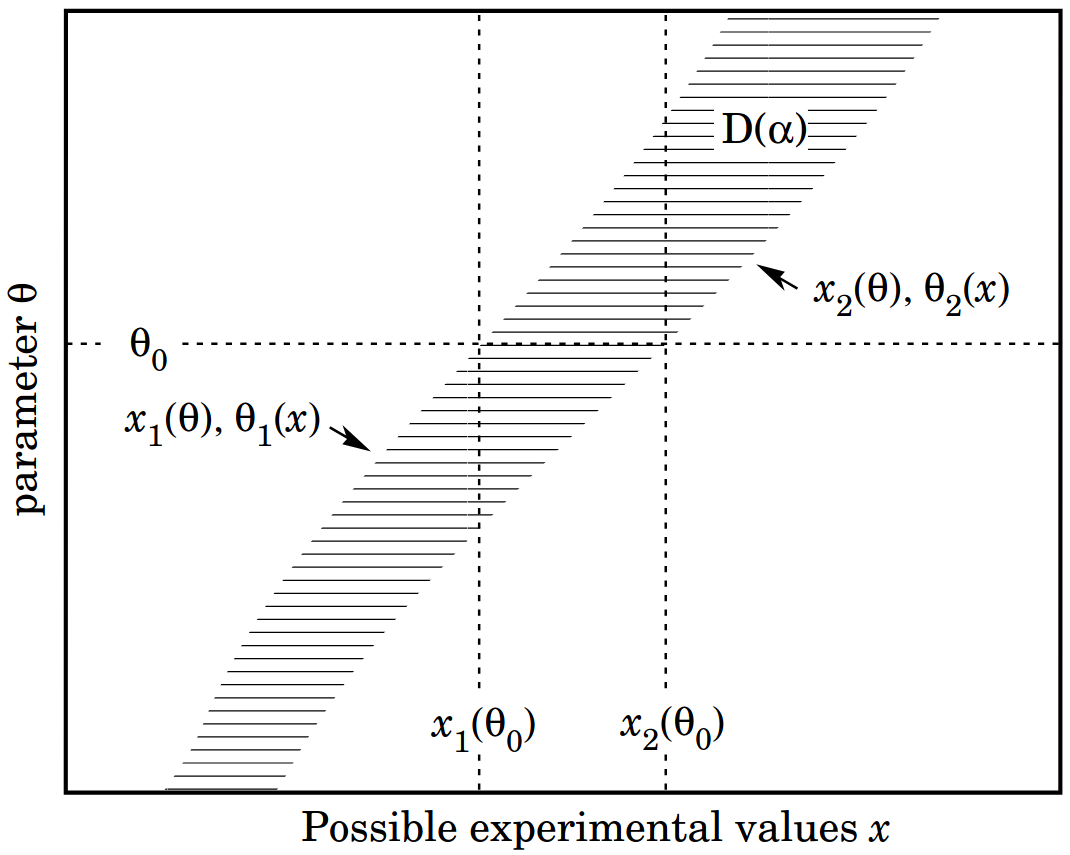
\includegraphics[width=\linewidth]{../plots/neyman.png}
\end{figure}
\end{minipage}
    
\end{frame}

\begin{frame}{Bayesian intervals}

Credible intervals $[\theta_l, \theta_u]$ cover $1-\alpha$ of the posterior
$$
1-\alpha = \int_{\theta_l}^{\theta_u} d\theta ~ p(\theta, x)
$$
\begin{itemize}
    \item For upper/lower limits: set $\theta_l$ or $\theta_u$ manually
    \item Highest (posterior) density intervals (HDI): smallest possible interval
\end{itemize}
\end{frame}

\begin{frame}{Example}
    % https://www.pp.rhul.ac.uk/~cowan/stat/beijing10/cowan_beijing10_5.pdf
    % https://pdg.lbl.gov/2024/reviews/rpp2024-rev-statistics.pdf

    \begin{itemize}
        \item Our independent data : $x_i, y_i, \sigma_i$
    \end{itemize}

    \begin{figure}
        \centering
        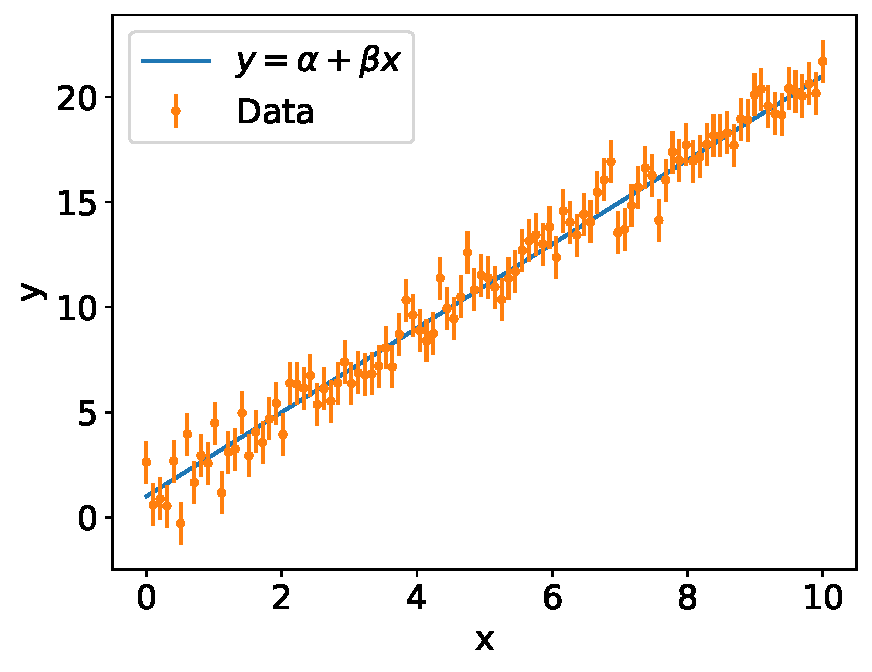
\includegraphics[width=0.5\linewidth]{../plots/linear_data.pdf}
    \end{figure}

\end{frame}

\begin{frame}{Example}
    \begin{itemize}
        \item Our independent data: $x_i, y_i, \sigma_i$
        \item Our model:
        $$ p(\mathbf{x}|\theta_0, \theta_1) = \prod_{x_i \in \mathbf{x}}\text{Gauss}(x_i | \mu(x_i|\theta_0, \theta_1), \sigma_i)$$
        $$\mu(x_i|\theta_0, \theta_1) = \theta_0 + \theta_1 x_i$$
         \item[\arrow] We want to know about $\theta_0$, do not care about $\theta_1$.
    \end{itemize}
\end{frame}

\begin{frame}{Likelihood}
\vspace{-1cm}
    $$ -2\log p(\mathbf{x}|\theta_0, \theta_1) = \sum_{x_i \in \mathbf{x}}\frac{\left(x_i -\mu(x_i|\theta_0, \theta_1)\right)^2}{\sigma_i^2}$$
    \begin{figure}
        \centering
        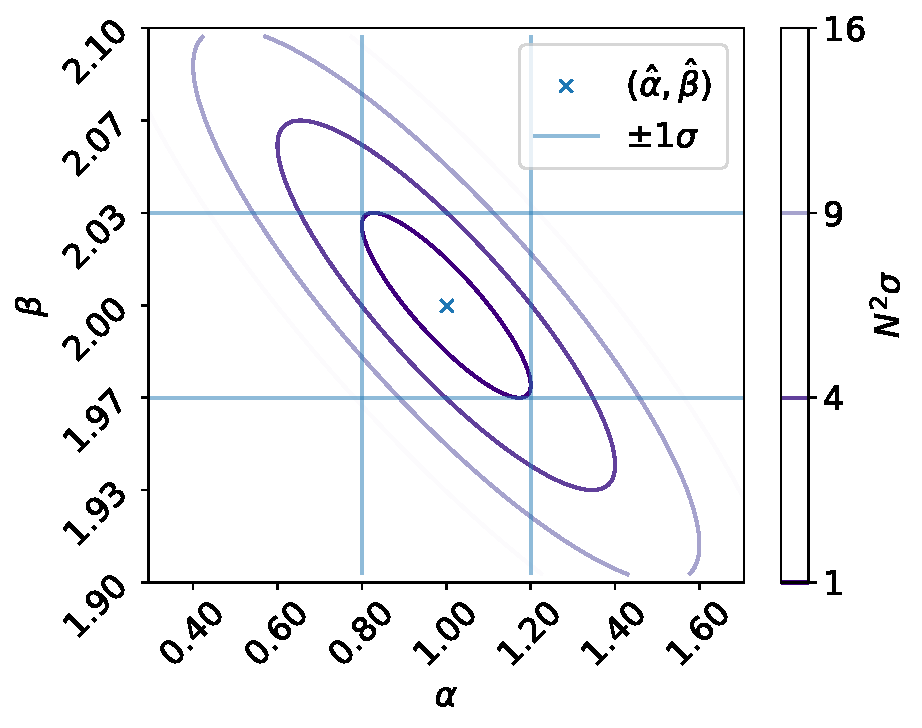
\includegraphics[width=0.5\linewidth]{../plots/nll_unconstr.pdf}
    \end{figure}
\end{frame}

\begin{frame}{Constrained likelihood}
\vspace{-1cm}
    $$ -2\log p(\mathbf{x}|\theta_0, \theta_1) = \sum_{x_i \in \mathbf{x}}\frac{\left(x_i -\mu(x_i|\theta_0, \theta_1)\right)^2}{\sigma_i^2} + \frac{\left(\theta_1 -t_1\right)^2}{\sigma_{t_1}^2} $$
    \begin{figure}
        \centering
        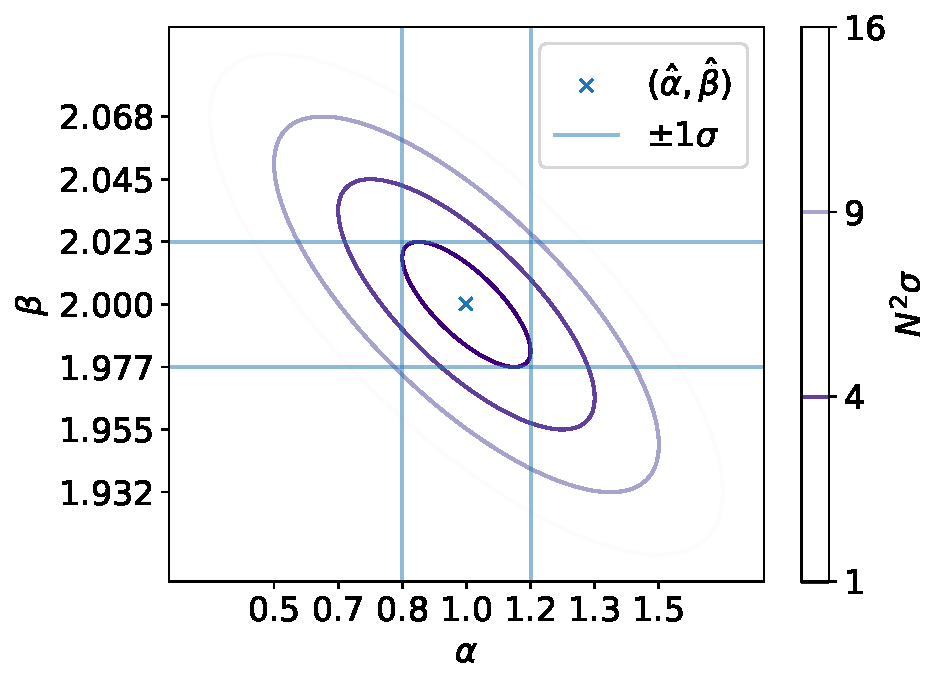
\includegraphics[width=0.5\linewidth]{../plots/nll_constr.pdf}
    \end{figure}
\end{frame}

\begin{frame}{Posterior}
\vspace{-1cm}
    $$p(\theta_0, \theta_1|\mathbf{x}) \propto p(\mathbf{x}|\theta_0, \theta_1) \pi(\theta_0)\pi(\theta_1)$$
    \begin{minipage}{0.49\linewidth}
        $$\pi(\theta_0) = \text{Uniform}(0,2)$$
        $$\pi(\theta_1) = \text{Gauss}(\theta_1 | t_1, \sigma_{t_1})$$
    \end{minipage}
    \begin{minipage}{0.49\linewidth}
    \begin{figure}
        \centering
        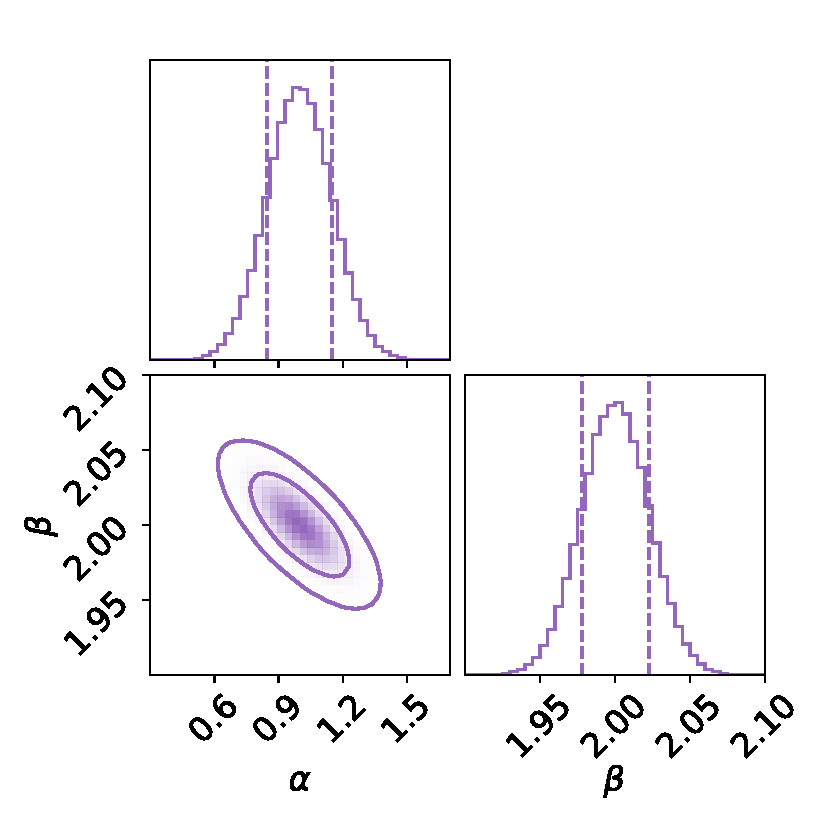
\includegraphics[width=0.9\linewidth]{../plots/posterior.pdf}
    \end{figure}
    \end{minipage}
\end{frame}

\begin{frame}{Marginal posterior}
\vspace{-1cm}
    $$p(\theta_0|\mathbf{x}) = \int d\theta_1 ~ p(\theta_0, \theta_1|\mathbf{x}) = \text{Gauss}(\theta_0 | \hat \theta_0, \sigma_{\theta_0})$$
    \begin{minipage}{0.49\linewidth}
    In this case, we get: 
        \begin{itemize}
            \item Same $\hat \theta_0$ as for ML
            $$
            \hat \theta_0 = 
            $$
            \item Same $\sigma_{\theta_0}$ as for ML
            $$
            \sigma_{\theta_0}^2 = \sum_{x_i,  \sigma_i\in \mathbf{x}, \mathbf{\sigma}}\sigma_{t_1}x_i^2 + \sigma_i^2
            $$
        \end{itemize}
    \end{minipage}
    \begin{minipage}{0.49\linewidth}
    \begin{figure}
        \centering
        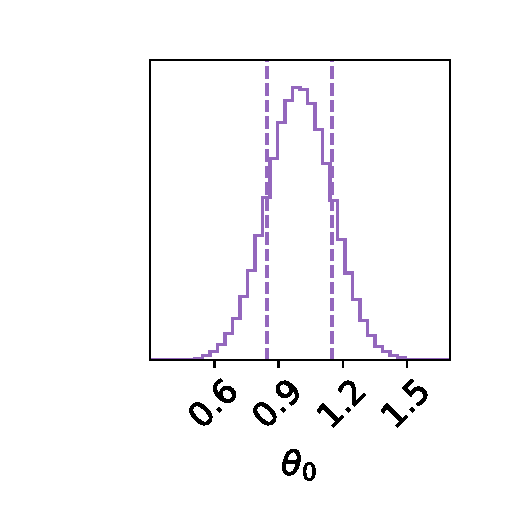
\includegraphics[width=0.9\linewidth]{../plots/marginal_posterior.pdf}
    \end{figure}
    \end{minipage}
\end{frame}

\begin{frame}
\center
\Large
MCMC
\end{frame}

\begin{frame}{The hard part ...}
\begin{itemize}
    \item Usually, we are not interested in the nuisance parameters $\nu$.
    \item One can obtain the posterior p.d.f. for $\theta$ alone by integrating over $\nu$.
    \item The \textit{marginal posterior} is 
        $$
        p(\theta | x) = \int d\nu ~ p(\theta, \nu | x)
        $$
    \item High dimensional integral \arrow compute with Monte Carlo methods.    
\end{itemize}
\end{frame}

\begin{frame}{Markov Chain Monte Carlo (MCMC)}
    \begin{figure}
        \centering
        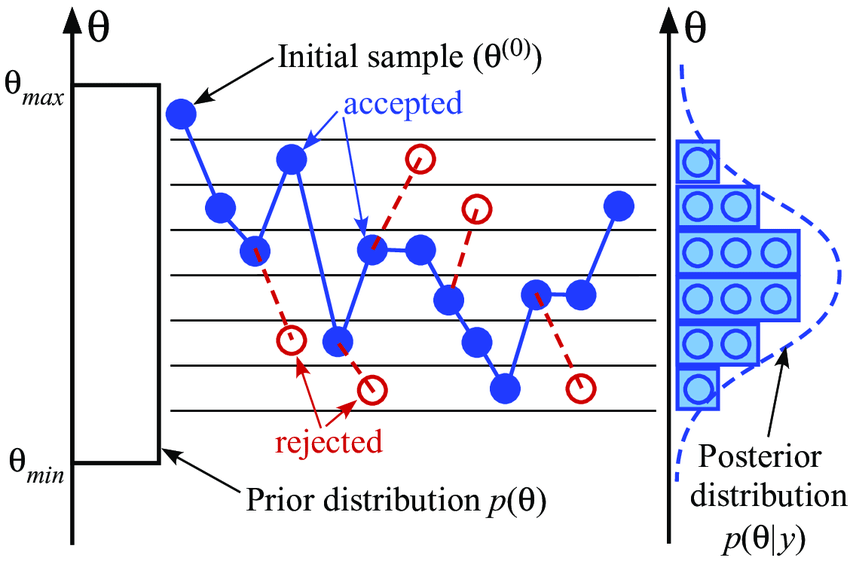
\includegraphics[width=0.6\linewidth]{../plots/mcmc_diagram.png}
    \end{figure}
    % https://doi.org/10.3390/app10010272
\end{frame}

\begin{frame}{Metropolis-Hastings}

\begin{enumerate}
    \item Generate $\theta \sim g(\theta|\theta_0)$
    \item Form Hastings test ratio $\alpha = \text{min}\left( \frac{p(\theta)g(\theta|\theta_0)}{p(\theta_0)g(\theta_0|\theta)}\right)$
    \item Generate $u \sim \text{Uniform}(0, 1)$
    \item If $u \leq \alpha$, let $\theta_1 = \theta$. Otherwise, let $\theta_1 = \theta_0$
    \item Set  $\theta_0 = \theta_1$ and return to step 1.
\end{enumerate}
    
\end{frame}

\begin{frame}{Chains}
    In MCMC we generate a sequence
    $$
    \theta_0 \to \theta_1 \to \theta_2 \to \ldots
    $$
    Only starting at one point can land you in local minima, hence often we sample
    \begin{align*}
        &\theta_0^0 \to \theta_1^0 \to \theta_2^0 \to \ldots \\
        &\theta_0^1 \to \theta_1^1 \to \theta_2^1 \to \ldots \\
        &\theta_0^2 \to \theta_1^2 \to \theta_2^2 \to \ldots \\
        &\ldots
    \end{align*}
\end{frame}

\begin{frame}{Convergence}
    Trace plots are a useful convergence diagnostic
    \begin{minipage}[t]{0.49\linewidth}
    \begin{figure}
        \centering
        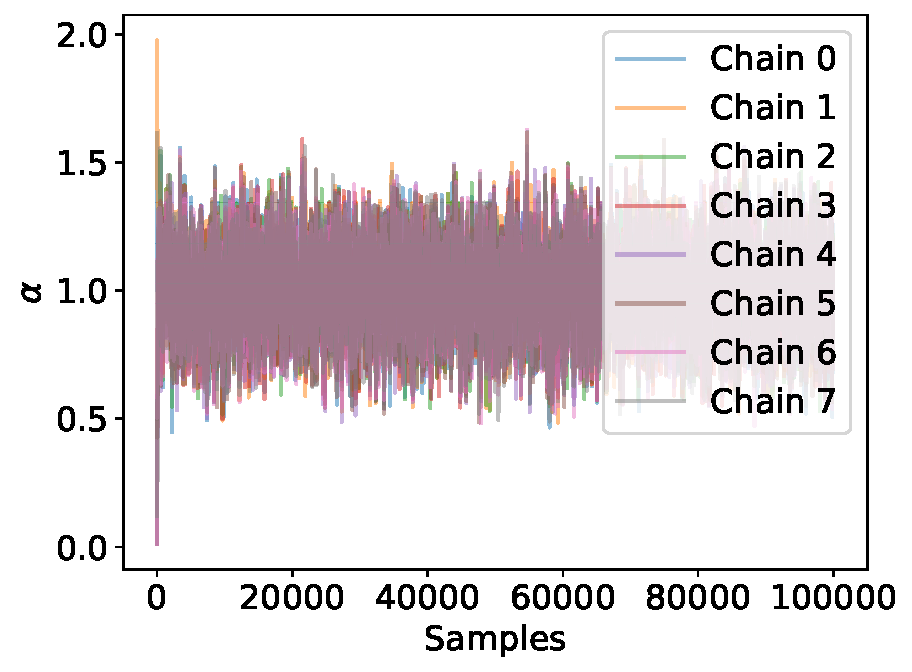
\includegraphics[width=\linewidth]{../plots/trace_theta0.pdf}
    \end{figure}
    \end{minipage}
    \begin{minipage}[t]{0.49\linewidth}
    \begin{figure}
        \centering
        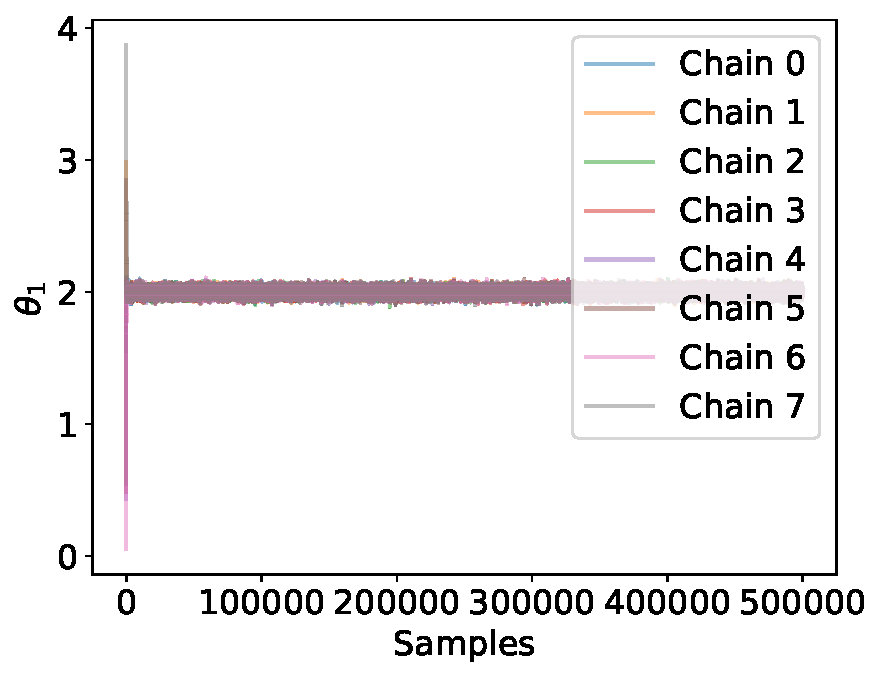
\includegraphics[width=\linewidth]{../plots/trace_theta1.pdf}
    \end{figure}
    \end{minipage}
    ... but one can become more fancy. %TODO reference
\end{frame}

\begin{frame}{Tools to try}
arviz, corner, pymc
\end{frame}

\begin{frame}{Exercises}

\textbf{a simple MCMC algorithm}\\

\end{frame}

\begin{frame}{Exercises: s+b problem}
\small
You do a binned analysis. You observe [155, 121,  13] in each bin respectively. From simulation, you expect to see [90, 30, 0] signal events (where the last bin acts as a control measurement) and [50, 70, 10] background events.\\
Hint: It is better to work with log-probabilities
    
\end{frame}

\begin{frame}{Exercises: s+b problem}
\small
\begin{itemize}
    \item Construct a likelihood function (chi2)
    \item What is the best fit point?
    \item What are the frequentist limits?
    \item What would a sensible choice of priors be for this example?
    \item Use an implementation of the Metropolis Hastings algorithm to sample from the posterior
    \item Make a corner plot of the posterior
    \item How do the mode of the posterior and the credible intervals compare to the best fit point and frequentist limits?
\end{itemize}
    
\end{frame}

%%%%%%%%%%%%%%%%%%%%%%%%%%%%%%%%%%%%%%%%%%%%%%%%%%%%%%%%%%%%%%%%%%%%%%%%%%%%%%%%%%%
\appendix

\begin{frame}
    \center
    \Large
    Solutions to exercises
\end{frame}



\end{document}


% https://drive.google.com/drive/folders/16CIMfhQkyEqMYkhLcsnzN0Yu5C2WHNU74

% https://pdg.lbl.gov/2024/reviews/rpp2024-rev-statistics.pdf

interested in using a given sample of data to make inferences about a probabilistic model

In Bayesian statistics, the subjective interpretation of probability is used to quantify one’s
degree of belief in a hypothesis. This allows one to define a probability density function (p.d.f.) for
a parameter, which reflects one’s knowledge about where its true value lies.

 hypothesis H is a statement about the probability for the data,
often written P (x|H)

If the probability P (x|H) for data x is regarded as a function of the hypothesis H, then it is
called the likelihood of H, usually written L(H). Often the hypothesis is characterized by one or
more parameters θ, in which case L(θ) = P (x|θ) is called the likelihood function.

In the Bayesian approach, inference is based on the posterior probability for H given the data
x, which represents one’s degree of belief that H is true given the data. 

Bayesian statistics supplies no unique rule for determining the prior.  it is important to carry out a sensitivity analysis, that is, to show how the result changes under a reasonable variation of the prior probabilities

For the special case of a constant prior, one can see from Bayes’ theorem (40.37) that the
posterior is proportional to the likelihood, and therefore the mode (peak position) of the posterior
is equal to the maximum-likelihood estimator. The posterior mode, however, will change in general
upon a transformation of parameter. One may use as the Bayesian estimator a summary statistic
other than the mode, such as the median, which is invariant under parameter transformation. But
this will not in general coincide with the MLE